\documentclass[a4paper,11pt,uplatex]{jsbook}
%\usepackage{fancyhdr}
\setlength{\footskip}{16pt}
\usepackage{amsmath}
\usepackage[dvipdfmx]{graphicx}
\usepackage[dvipdfmx]{color}
%\usepackage{pagecolor}[white]
\usepackage{amsmath,amssymb}
%\usepackage[top=3cm, bottom=3cm, left=3cm, right=3cm]{geometry}
\usepackage{braket}
\usepackage{bm}
\numberwithin{equation}{section}
\usepackage{mathrsfs}
\usepackage{siunitx}
\usepackage{physics}
\usepackage[dvipdfmx]{graphicx}
\usepackage[compat=1.1.0]{tikz-feynhand}
\usepackage{caption}
\usepackage{subcaption}
%\usepackage{cleveref}
\usepackage{float}
\usepackage{multicol}
\setlength{\columnsep}{15mm}
%\usepackage[style=phys,articletitle=false,biblabel=brackets,chaptertitle=false,pageranges=false]{biblatex}
%\usepackage[style=phys]{biblatex}
\usepackage[dvipdfmx]{hyperref}
\usepackage{url}
\usepackage{pxjahyper}
\usepackage{bookmark}
%\usepackage[backref]{hyperref}
\setcounter{tocdepth}{3}
\setlength{\parindent}{2em}
\def\vector#1{\mbox{\boldmath $#1$}}
\def\slash#1{\not\!#1}
\def\slashb#1{\not\!\!#1}
\def\delsla{\not\!\partial}
\usepackage[dvipdfmx]{xcolor}


\hypersetup{
 setpagesize=false,
 bookmarksnumbered=true,%
 bookmarksopen=true,%
 colorlinks=true,%
 linkcolor=black,
 citecolor=red,
 urlcolor=black,
}
%backreferenceのカスタマイズ. "Back to p.3"のように表示する.
%\renewcommand*{\backref}[1]{(p.#1へ戻る)}
%\newcommand{\backtoc}{\hyperlink{toc}{[目次へ]}}
\newcommand{\backtoc}{\texorpdfstring{\protect\hyperlink{toc}{\hspace{5pt} \scriptsize [目次へ]}}{}}
\newcommand{\mychapter}[1]{\chapter[#1]{#1\backtoc}}
\newcommand{\mysection}[1]{\section[#1]{#1\backtoc}}
\newcommand{\mysubsection}[1]{\subsection[#1]{#1\backtoc}}

% 数式
%\usepackage{amsmath,amsfonts}
%\usepackage{bm}
%\usepackage{physics}
% 画像
%\usepackage[dvipdfmx]{graphicx}
%\usepackage[dvipdfmx,colorlinks=true,linkcolor=blue]{hyperref}
%\usepackage{pxjahyper}

\begin{document}

\chapter{データ解析と結果}
この章ではデータ解析の手順と結果について述べる。

単独アンジュレータのデータおよびエネルギー測定用の2台のアンジュレータのデータの2つのデータセットがある。
画像処理までの手順は共通であるのでまずは画像処理について述べる。
続いて単独アンジュレータのデータの解析結果を述べる。
最後に2台のアンジュレータのデータの解析結果について述べる。\\
なおエネルギー測定のデータセットは以下のように構成されている。
\begin{itemize}
  \item 水銀灯の波長較正データ1枚
  \item アンジュレータの位置データ 166個の値
  \item 干渉光の画像データ 166 position $\times$ 4 画像 = 664枚
\end{itemize}
これを反映し、エネルギーデータ解析の手順は以下のようになる。
\begin{enumerate}
  \item 波長較正:ピクセル-波長直線を求める
  \item 画像の統合:664枚$\rightarrow$ 166枚の二次元データ
  \item 較正波長でのデータの切り出し:166枚の二次元データ $\rightarrow$ 166個の1次元データ
  \item モデル関数によるフィッティング
\end{enumerate}

\section{画像処理}
\noindent \textbf{\underline{解析}}\par
各ピクセルにおける発光量に対応して、0から65535(16~bit)の整数値が割り当てられる。この値をピクセル値と定義する。

まず電子ビームを入射していない状態の画像を取得し、これを背景画像とする。露光時間1 秒で10枚の画像を連続で取得し、各ピクセルごとにピクセル値の平均値を計算し、背景画像とする。

各runでは、各ピクセルごとに同一条件(アンジュレータ位置、波長などの条件)で4枚の画像が取得される。
これらの4枚の画像について、各ピクセルごとにピクセル値の平均値を取り、代表値とする。
またピクセルの誤差は4枚の画像におけるピクセル値の標準偏差とする。

予想される回折パターンの性質を考えると、隣り合うピクセル同士の発光量の差は周囲の上下左右のピクセルに対して極端に発光量が多いピクセルはノイズであると判断してマスクし、フィッティングの対象に含まない。

\noindent \textbf{\underline{結果}}\par
あるピクセルにおける、4枚の画像のピクセル値の平均値と標準偏差の関係を図\ref{pixel}に示す。
\begin{figure}[h]
  \centering
  \includegraphics[width=0.8\linewidth]{image/4-pixel.png}
  \caption{ピクセルの平均値と標準偏差の関係}\label{pixel}
\end{figure}
ピクセルの発光量はポアソン分布に従うことから、標準偏差は平均値の平方根に比例すると考えられる。
オフセットを考慮してフィッティングした結果、平均値と標準偏差の関係は
\begin{eqnarray}
  \text{標準偏差} = 0.298(4) \sqrt{\text{平均値} - 79.2(1.6) } 
\end{eqnarray}
となった。

背景画像の結果を図\ref{BG}に示す。発光量が極端に多いノイジーなピクセルが見られるが、ピクセル値が150以上のピクセルは150に置き換えて表示している。
\begin{figure}[h]
  \centering
  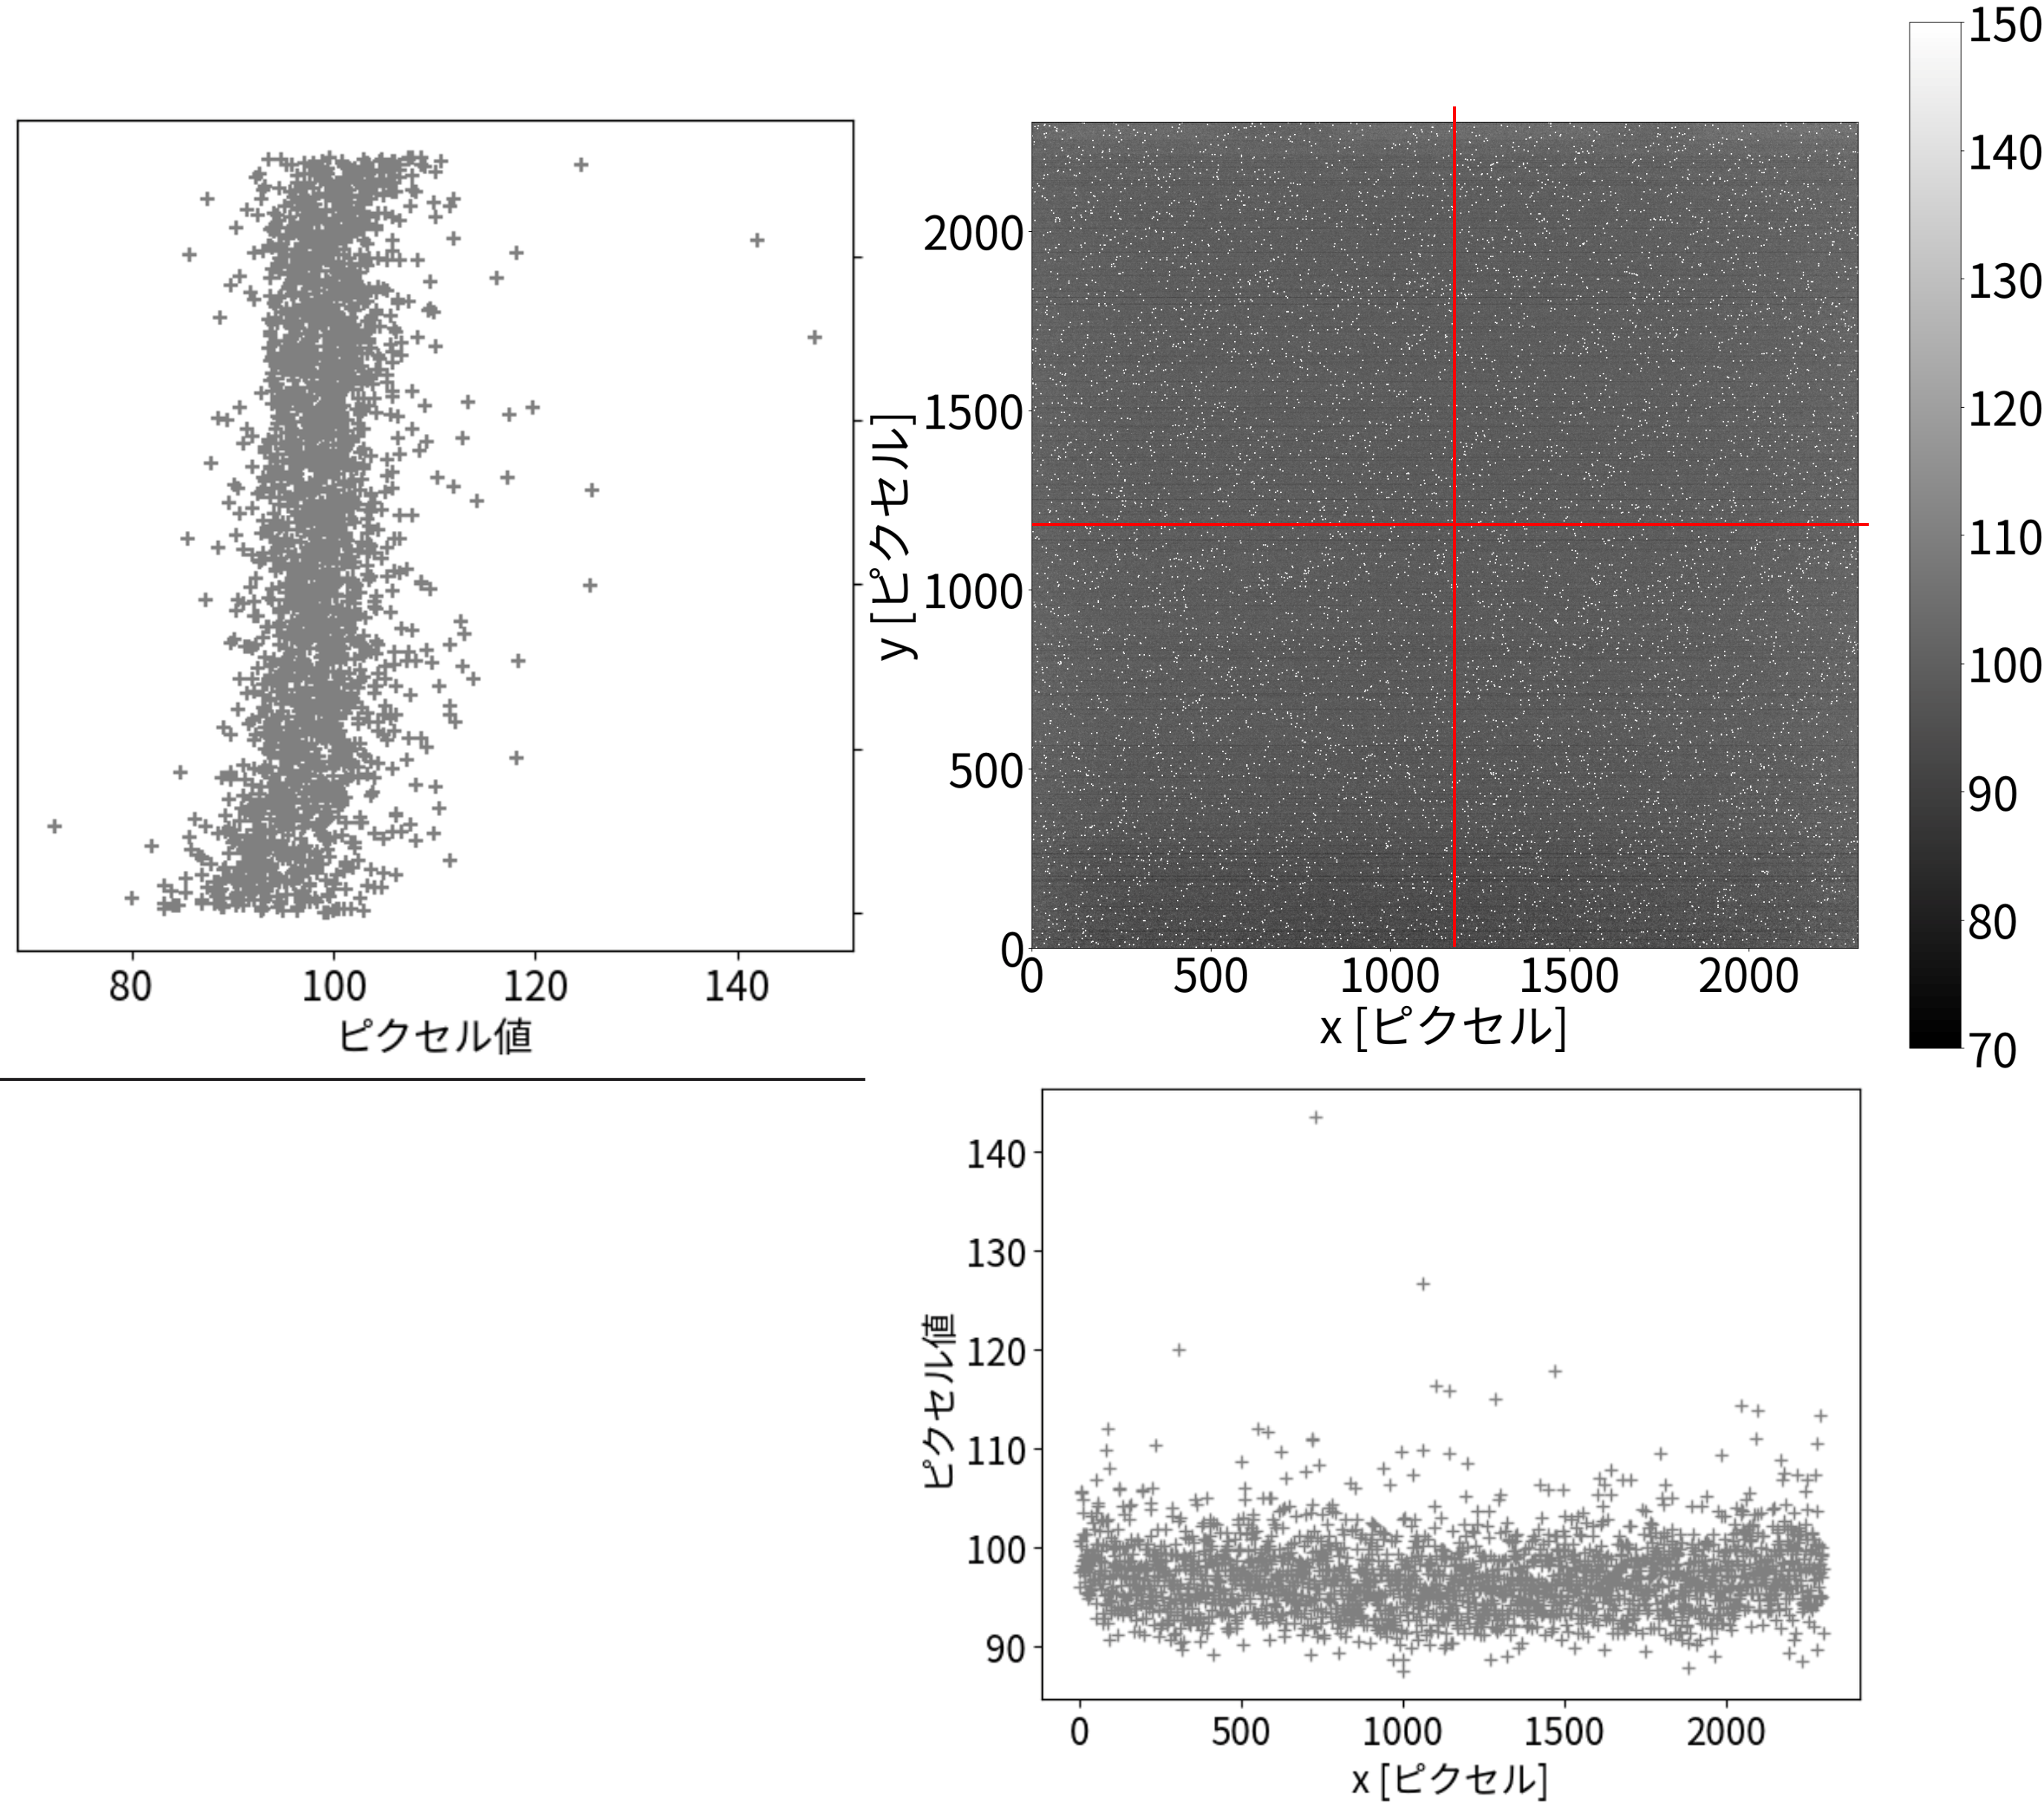
\includegraphics[width=0.8\linewidth]{image/4-BG.png}
  \caption{背景画像。ピクセル値が150以上のピクセルは150に置き換えて表示している。}\label{BG}
\end{figure}
背景画像のピクセル値の分布を図\ref{BGmean}に示す。全画素にわたるピクセル値の平均値は98.91、標準偏差は4.57であった。ピクセル値が150以上のピクセルは全体の0.14 \%であった。
\begin{figure}[b]
  \centering
  \begin{subfigure}[b]{0.33\linewidth}
    \centering
    \includegraphics[width=\linewidth]{image/4-BGmean.png}
    \subcaption{150以下の平均値分布}
  \end{subfigure}
  \hfill
  \begin{subfigure}[b]{0.33\linewidth}
    \centering
    \includegraphics[width=\linewidth]{image/4-BGmeanlog.png}
    \subcaption{150 以下の平均値分布(対数表示)}
  \end{subfigure}
  \hfill
  \begin{subfigure}[b]{0.33\linewidth}
    \centering
    \includegraphics[width=\linewidth]{image/4-BGmeanall.png}
    \subcaption{平均値の全分布}
  \end{subfigure}
  \caption[背景画像の光量分布]{背景画像のピクセルの平均値分布}
\end{figure}



\begin{figure}
  \centering
  \includegraphics[width=0.8\linewidth]{image/4-BGmean.png}
  \caption{背景画像のピクセル値の平均値分布}\label{BGmean}
\end{figure}


全てのピクセルの平均値と標準偏差の関係を示す。

周囲のピクセルと比較した超過値の分布を示す。閾値として今回は40を設定した。超過値が40を超えるピクセルはノイズピクセルとして除去した。
ノイズピクセルと判定されたピクセルの割合は平均して??\%であった。
また、ピクセルが異常を起こし、常にノイズピクセルとして判定される割合は??\%程度だったのに対し、放射線など偶発的にノイズが乗るピクセルは??\%程度であった。
\subsection{平滑化}
画像の平滑化が必要な場合には、波長方向にのみ行う。同様にノイズピクセルをマスクしたうえで、マスクされなかったピクセルの平均値と標準偏差を計算し、ピクセルの誤差は標準偏差を計算に用いたピクセルの数の平方根で割った値(標準誤差)とする。

\section{波長較正}
\noindent \textbf{\underline{解析}}\par
水銀灯の404.656 nmおよび407.781 nmの輝線スペクトルを取得する。画像の$y$軸方向に50 ピクセルのカットをかけた1次元データを取得し、ガウシアンによるフィッティングを行う。
フィッティングで得られたピークの中心値と波長から、ピクセル-波長関係を求める。
ピークの中心決定精度から波長較正の精度を求める。

\noindent \textbf{\underline{結果}}\par
水銀灯の波長較正で得られた画像の例を図\ref{mercury}に示す。
\begin{figure}[h]
  \centering
  \includegraphics[width=0.8\linewidth]{image/4-mercury.png}
  \caption[水銀灯の波長較正-1]{水銀灯の波長較正で得られた画像。404.656 nmと407.781 nmに対応する輝線が見える。この輝線スペクトルをもとにピクセル-波長関係から得られた波長の値が画像の上の軸である。}\label{mercury}
\end{figure}
$y$軸方向に50 ピクセルのカットをかけて、ガウシアンによるフィッティングを行った結果を図\ref{mercuryfit}に示す。
輝線スペクトルの中心付近でのカットの結果、中心値のピクセルとフィットによる中心決定精度は
\begin{eqnarray}
  ピクセル_{404.7} &=& 1209.5912(9)\\
  ピクセル_{407.8} &=& 1868.155(4) 
\end{eqnarray}
と求められた。これらの値を元に、ピクセル-波長関係が求められる。特に1 ピクセルあたりの波長分散は、
\begin{eqnarray}
  \lambda / ピクセル = 0.0047~\text{nm}
\end{eqnarray}
である。また、輝線スペクトルの幅($\sigma$)は404.656 nmのピークが3.5 ピクセル、407.781 nmのピークが2.1 ピクセルと見積もられているが、これはそれぞれ0.0016 nm、0.0010 nmの波長分散に相当し、
較正波長約400 nm に対して$10^{-4}$以下に抑えられている。
\begin{figure}[h]
  \centering
  \begin{subfigure}[h]{0.33\linewidth}
    \centering
    \includegraphics[width=\linewidth]{image/4-fpeak.png}
    \subcaption{404.656 nmのピーク}
  \end{subfigure}
  \hfill
  \begin{subfigure}[h]{0.33\linewidth}
    \centering
    \includegraphics[width=\linewidth]{image/4-speak.png}
    \subcaption{407.781 nmのピーク}
  \end{subfigure}
  \hfill
  \begin{subfigure}[h]{0.33\linewidth}
    \centering
    \includegraphics[width=\linewidth]{image/4-bothpeak.png}
    \subcaption{2つのピーク}
  \end{subfigure}
  \caption[水銀灯の波長較正-2]{水銀灯のデータをガウシアンでフィッティングした結果。フィッティングパラメータの中心値および標準偏差$\sigma$の結果を判例に示した。これらの数値に付けられている誤差はフィッティングの誤差を表す。}
\end{figure}\label{mercuryfit}

次に水銀灯の輝線がカメラに対してどの程度傾いているかを調べた。
$y$軸方向のカットをかけるピクセルを輝線が明瞭に見える$y$ = 700 ピクセルから$y$ = 1800 ピクセルの範囲で変えてガウシアンフィッティングを行い、ピークの中心値の依存性を調べた結果を図\ref{tiltfit}に示す。
2つのピークで中心値の傾きは線形で近似可能であり、これは光軸に対してカメラが傾いている効果で説明可能である。
またその傾きは線形フィットによれば
\begin{eqnarray}
  x方向の変位 / y軸方向の変位 = 5 \times 10^{-3}
\end{eqnarray}
程度に抑えられており、カメラの上下2304 ピクセルに対して約12ピクセルの変位が生じることがわかる。
1ピクセルあたりの波長分散は0.0047~nmであるからこれは0.05~nmに相当する。
しかし、発光量の多い領域は高々1500 ピクセル程度の範囲に限られており、この領域における波長分散は最大0.035~nm程度と見積もられる。
式(\label{zero order energy formula}) $\text{E}_\text{beam} =m_e c^2  \sqrt{\lambda_{\text{osc}}/2\lambda_L} $によって、波長決定精度がエネルギー決定精度に与える影響を見積もると、$\delta \text{E}_\text{beam}/\text{E}_\text{beam} = \delta \lambda_L/\delta \lambda_L$であり、
ここに較正波長$\lambda_L \sim 400~\text{nm}$、$\delta \lambda_L \sim 0.0035~\text{nm}$を代入すれば
カメラの傾きによる波長分散の効果は$10^{-4}$以下に抑えられていると言える。
\begin{figure}[h]
  \centering
  \begin{subfigure}[h]{0.3\linewidth}
    \centering
    \includegraphics[width=\linewidth]{image/4-tilt.png}
    \subcaption{輝線の傾きの図示}
  \end{subfigure}
  \hfill
  \begin{subfigure}[h]{0.3\linewidth}
    \centering
    \includegraphics[width=\linewidth]{image/4-tiltfpeak.png}
    \subcaption{404.656 nmのピーク}
  \end{subfigure}
  \hfill
  \begin{subfigure}[h]{0.3\linewidth}
    \centering
    \includegraphics[width=\linewidth]{image/4-tiltspeak.png}
    \subcaption{407.781 nmのピーク}
  \end{subfigure}
  \caption[水銀灯の波長較正-3]{輝線スペクトルの傾きの解析結果。$y$軸方向に50 ピクセルのカットをかける範囲を変えてガウシアンフィッティングを行い、その中心値をプロットした。2つのピークに対して$y$-ガウシアンの中心関係を線形フィットして得られた傾きの値を凡例に示した。}\label{tiltfit}
\end{figure}

\section{モデル関数によるフィッティング}
\noindent \textbf{\underline{解析}}\par
この節では、単独アンジュレータのデータおよび2台のアンジュレータのデータ両方の解析に用いるモデル関数について述べる。モデル関数は、エネルギーを含む各種パラメータとアンジュレータの位置を入力として、回折パターンの形状をカメラの$y$座標の関数として出力する関数である。
\subsection{1電子放射光関数}
アンジュレータ放射光の振幅は放射角の関数として式(\ref{eq:spectrum})のように計算できる。
また放射光の位相は、アンジュレータの位置を光源とする球面波位相として計算する。
\subsection{フレネル回折}
放射光関数で計算されたスリットにおける光波($U(x)$)から、カメラにおける回折光を計算する。
\subsubsection{数値計算上の計算手法}
数値計算を実行する上では数値積分の手法では、伝搬後の$N$次元の配列が伝搬前の$N$次元配列全ての積分を用いて計算されるため計算量は$N^2$となる。
このような計算コストの高い計算を避けるために、高速フーリエ変換を用いた計算が一般に用いられている。
式(\ref{レイリーゾンマーフェルト近似})を再度$x,y,x_0,y_0$で書き直すと
\begin{eqnarray}
  U(x_0,y_0) \sim \frac{1}{2i\lambda zs}\int_S U(x,y) \exp( ik \sqrt{z^2 + (x-x_0)^2 + (y-y_0)^2}) dxdy
\end{eqnarray}
これはカーネル関数$f(x,y) = \sqrt{z^2 +x^2 + y^2}$であるような畳み込みの形で書ける。
\begin{eqnarray}
  U(x_0,y_0) \sim (U * f)(x,y)
\end{eqnarray}
畳み込みはフーリエ変換を用いることで
\begin{eqnarray}
  (U*f)(x,y) = \mathcal{F}^{-1}(\mathcal{F}(U) \times \mathcal{F}(f)) \label{convolution}
\end{eqnarray}
と表せる。ここで$\mathcal{F}$はフーリエ変換を表す。これは以下のように示すことができる。
\begin{eqnarray}
  (U*f)(x) = \int_{-\infty}^{\infty} U(t)f(x-t)dt
\end{eqnarray}
これをフーリエ変換したものは、
\begin{eqnarray}
  \mathcal{F}(U*f)(k) = \int_{-\infty}^{\infty} \int_{-\infty}^{\infty} U(t)f(x-t)dt \exp(-ikx)dx
\end{eqnarray}
積分の順序を交換して$x-t = y$とおくと、
\begin{eqnarray}
  \mathcal{F}(U*f)(k) &=& \int_{-\infty}^{\infty} U(t) \exp(-ikt)dt \int_{-\infty}^{\infty} f(y) \exp(-iky)dy\\
  &=& \mathcal{F}(U) \times \mathcal{F}(f)
\end{eqnarray}
したがって式(\ref{convolution})が示される。

フーリエ変換による計算では、空間領域($x,y$)の光波を周波数領域($k_x,k_y$)に変換する場合、空間領域の光波は計算に用いた空間領域を1周期とする周期的な光波として扱われている(図\ref{ft}(a))。そのため、そのまま逆変換を行うと隣り合う空間領域の光波が干渉してしまい、いわゆる円状畳み込みの結果を与える。これを防ぐために、計算空間の端を0で埋めた上で計算に用いる空間領域を拡大するゼロパディングを行うことで、(直線状)畳み込みの結果を得ることができる(図\ref{ft}(b))。
\begin{figure}
  \centering
  \begin{subfigure}[h]{0.3\linewidth}
    \centering
    \includegraphics[width=\linewidth]{image/4-ft.png}
    \subcaption{円状畳み込み}
  \end{subfigure}
  \hfill
  \begin{subfigure}[h]{0.65\linewidth}
    \centering
    \includegraphics[width=\linewidth]{image/4-ft_zeropadding.png}
    \subcaption{ゼロパディング}
  \end{subfigure}
  \caption[フーリエ変換による畳み込みの数値計算]{フーリエ変換による畳み込みの数値計算。左図のように周波数領域では周期的な光波として扱われている。そのため、畳み込みを行うと隣り合う空間領域が干渉しあう。ゼロパディングを行うとこの干渉を抑制することができる。}
\end{figure}\label{ft}

\subsection{電子ビームサイズ}
1電子の放射光であると仮定していた放射光関数は、電子ビームサイズを考慮すると、異なる電子からの放射光関数の重ね合わせとして表現できると考えられる。
$y$軸方向のビームサイズを$\sigma_y$としてガウス状の広がりを仮定し、放射光関数をこのガウシアンで畳みこむ。
これにより1電子放射光関数から得られる回折パターンはぼやける。電子ビームサイズによって回折パターンがぼやける様子を計算で再現した結果を図\ref{beamsize}に示す。
\begin{figure}
  \centering
  \includegraphics[width=0.8\linewidth]{image/4-esize.png}
  \caption[電子ビームサイズによる回折パターンのぼやけ]{電子ビームサイズによる回折パターンのぼやけ。畳み込みがない場合(灰色)と比較して
  ビームサイズの効果を入れた赤、緑、青の線は回折の微細構造がぼやけている}\label{beamsize}
\end{figure}

%\subsection{光学系}
%回折格子によって分光された光はレンズによってカメラで収束する。スリットの形状および回折格子はx方向にも幅を持つが、計算時間の都合上y軸方向のみの1次元の計算を行う。
%1次元の回折と2次元の回折の結果はほとんど変わらないことが確認されている。
\subsection{パラメータ}
モデル関数は、波長、カメラの$y$座標、アンジュレータの位置の関数として表現される。
これらの変数を表\ref{tab:variables}に示す。
\begin{table}[h]
  \centering
  \begin{tabular}{c|c}
    $\lambda_L$ & 観測光の波長。波長較正によってカメラの$x$軸と波長の関係が求められている。\\
    $y$ & カメラにおける$y$座標。カメラのチップサイズ14.976~mmに対応して-74.88 mm から74.88 mmの値をとる\\
    $d$ & アンジュレータの最上流を0と定義し、下流方向を正にとる。0 - 825 mmの値をとる\\
  \end{tabular}
  \caption[変数の定義]{変数の定義}\label{tab:variables}
\end{table}
モデル関数で出力される放射光の形状を制御するパラメータの定義を表\ref{tab:prm}および図\ref{prm}に示す。

\begin{table}[h]
\centering
\begin{tabular}{c|c}
  $\gamma$ & 電子ビームエネルギーのローレンツ因子 \\
  $K$ & アンジュレータの偏向定数 \\
  $z(U1-slit)$ & 下流アンジュレータ-スリット間の距離\\
  $z(U2-slit)$ & 下流アンジュレータ-スリット間の距離 \\
  $z(slit-cam)$ & スリット-カメラ間の距離 \\
  $w(slit)$ & スリットの鉛直方向の長さ \\
  $y(beam)$ & カメラに対するビーム中心の$y$座標 \\
  $y(slit)$ & カメラに対するスリット中心の$y$座標 \\
  $\delta \phi$ & 上流と下流のアンジュレータ放射の位相のずれ\\
  ampl & 光量にかかる比例係数
\end{tabular}
\caption[パラメータの説明]{パラメータの説明}\label{tab:prm}
\end{table}
\begin{figure}[h]
  \centering
  \includegraphics[width=0.8\linewidth]{image/4-prm.png}
  \caption[パラメータの定義]{パラメータの定義。アンジュレータ、光学系、
  ビーム同士の幾何学的な位置関係に関するパラメータを示した。}\label{prm}
\end{figure}
上流と下流のアンジュレータ放射の位相差は電子がアンジュレータ間を移動するのにかかる時間に比例する。
この時間はアンジュレータ間の距離に比例するのではなく、電子がアンジュレータ内で蛇行することによる平均の速度も影響するため、
$\delta \phi$というパラメータで位相差を調整する。


\subsection{パラメータ較正}
単独アンジュレータのデータを解析し、$z(U2- slit),z(slit-cam),w(slit)$の最適値を求める。
2台のアンジュレータのデータではこれらのパラメータを固定してフィッティングを行う。ただし系統誤差を見積もるために、パラメータを変化させた場合のフィッティングも行う。\\
また、アンジュレータが下流に移動することによる光量の変化をampl パラメータの$d$依存性に押し込む。この依存性から、上流アンジュレータと下流アンジュレータの寄与の係数も決定できる。
\section{単独アンジュレータの解析}
\noindent \textbf{\underline{解析}}\par
パラメータ較正を目的とした単独アンジュレータのデータの解析を述べる。
下流アンジュレータのみの磁場によって得られるデータから、放射光関数の位置依存性の情報が抽出できる。
理想的な条件では、アンジュレータが下流に移動すると以下のような変化が見られると考えられる。
\begin{itemize}
  \item アクセプタンスの増加による振幅の増加
  \item 光学的な位置関係の変化による回折パターンの形状の変化
\end{itemize}

振幅の上昇と回折パターンの形状の変化から、距離のパラメータ $z(U2-slit),z(slit-cam),w(slits)$の最適値を求めることができる。
$z(U2-slit),z(slit-cam),w(slit)$を固定してフィッティングを行い、適合度がもっとも良いパラメータの組を最適な値として定義する。

\noindent \textbf{\underline{結果}}\par
電子ビームエネルギー210 MeVにおいて取得した単独アンジュレータのデータを解析した。
%\subsubsection{波長依存性}
%波長依存性があり長波長側の光量が大きい傾向がある。
%この傾向は線形の依存性が仮定できる。\\
\subsubsection{位置依存性}
アンジュレータが下流に移動することによる回折パターンの変化を図\ref{DCposdep}に示す。上流側のパターンと比較すると、下流側($d= 825$)の回折パターンは振幅が大きくなり、回折パターン全体の幅が広がっていることがわかる。
また回折パターンは上流下流にかかわらず8つのピークがあるが、ピーク同士の相対的な高さの変化も見られる。
\begin{figure}
  \centering
  \includegraphics[width=0.8\linewidth]{image/4-DCposdep.png}
  \caption[アンジュレータ位置依存性]{単独アンジュレータデータの位置依存性。アンジュレータが最上流(赤)と最下流(青)に移動したときの回折パターンを比較すると、振幅やパターン全体の幅、回折のピーク同士の高さが変化していることがわかる。}\label{DCposdep}
\end{figure}

回折パターンの形状の変化はモデル関数において、放射光関数の球面波位相が変化することで説明できると考えられる。
振幅の変化は、$ampl$パラメータを$d$によって変化するパラメータ$ampl(d)$としてフィッティングを行うことで詳しく調べられる。フィッティングをおこない$ampl$パラメータを$d$に対してプロットした結果を図\ref{DCampl}に示す。
$d$に対して全体的に上昇する傾向と、周期的に変動する傾向が見られる。この周期的変動は約135~mmであり、
測定に用いた電子ビームエネルギー210 MeVに対応する周期的変動の周期(式(\ref{eq:energy_prim}))$\lambda_{osc} = 2\gamma^2\lambda_L \simeq 135~\text{mm}$に一致している。
これはアンジュレータ放射光と可干渉で、$d$に依存しない位相の光波が入射しており、この光波と下流アンジュレータの放射光の
相対的な位相が$d$に依存して変化していると考えられる。偏向電磁石によるシンクロトロン放射はこの条件を満たしており、
アンジュレータ下流の偏向電磁石による放射が単独アンジュレータの放射光の観測では無視できない。

また、振幅の上昇が、アクセプタンスの増加によるものだと仮定すると、振幅は見込む立体角に比例すると近似できるから、
$d$依存性は$1/z(U2-slit)^2$を反映したものになると考えられる。これらの仮定を踏まえて
\begin{eqnarray}
  ampl(d) = \frac{1}{(d - z(U2-slit))^2} + \sin\left( \frac{2\pi}{\lambda'_{osc}}d + \phi \right)\label{eq:ampl}
\end{eqnarray}
というモデル関数を用いてフィッティングを行うと、$z(U2-slit) = 10.51$ m、$\lambda_{osc}= 135.33$ mmという値が得られた。

\begin{figure}[h]
  \centering
  \includegraphics[width=0.8\linewidth]{image/4-DCampl.png}
  \caption[アンジュレータ位置依存性]{アンジュレータ位置に対する$ampl$パラメータの変化。アンジュレータが下流(D=825 側)に移動すると振幅が増加すると
  ともにおよそ135~mm周期で振動する傾向が見られる。}\label{DCampl}
\end{figure}

下流アンジュレータの$1/(z(U2-slit))^2$の依存性を外挿し、上流アンジュレータに対応する$ampl$パラメータも決定できる。
2台のアンジュレータの解析では、$ampl(d)$パラメータを用いてフィッティングを行う。

\section{2台のアンジュレータの解析}
\noindent \textbf{\underline{解析}}\par
パラメータ較正によって決定したパラメータを用いて2台のアンジュレータのデータを解析する。動かすパラメータは以下の通りである。
\begin{table}[h]
\centering
\begin{tabular}{cc}
  $\gamma$ & 電子ビームエネルギーのローレンツ因子 \\
  $y(beam)$ & カメラに対するビーム中心の$y$座標 \\
  $y(slit)$ & カメラに対するスリット中心の$y$座標 \\
  $\delta \phi$ & 上流と下流のアンジュレータの位相のずれ\\
  ampl & 振幅
\end{tabular}
\end{table}

これらのパラメータを動かしてモデル関数によるデータのフィッティングを行う。
フィッティングは既約カイ二乗値による最小二乗法を用いる。
またpythonのlmfitパッケージ\cite{lmfit}を用いてフィッティングを行う。\\
フィッティングで得られた$\gamma$の値から電子ビームエネルギーを求める。

\noindent \textbf{\underline{結果}}\par
図\ref{images}に2台のアンジュレータで得られる画像の例を示す。アンジュレータの位置$d$によって回折パターンの形状が変化することがわかる。波長によって振動の初期位相が違うため、強弱が長波長側に移動していくように見える。
\begin{figure}[h]
  \centering
  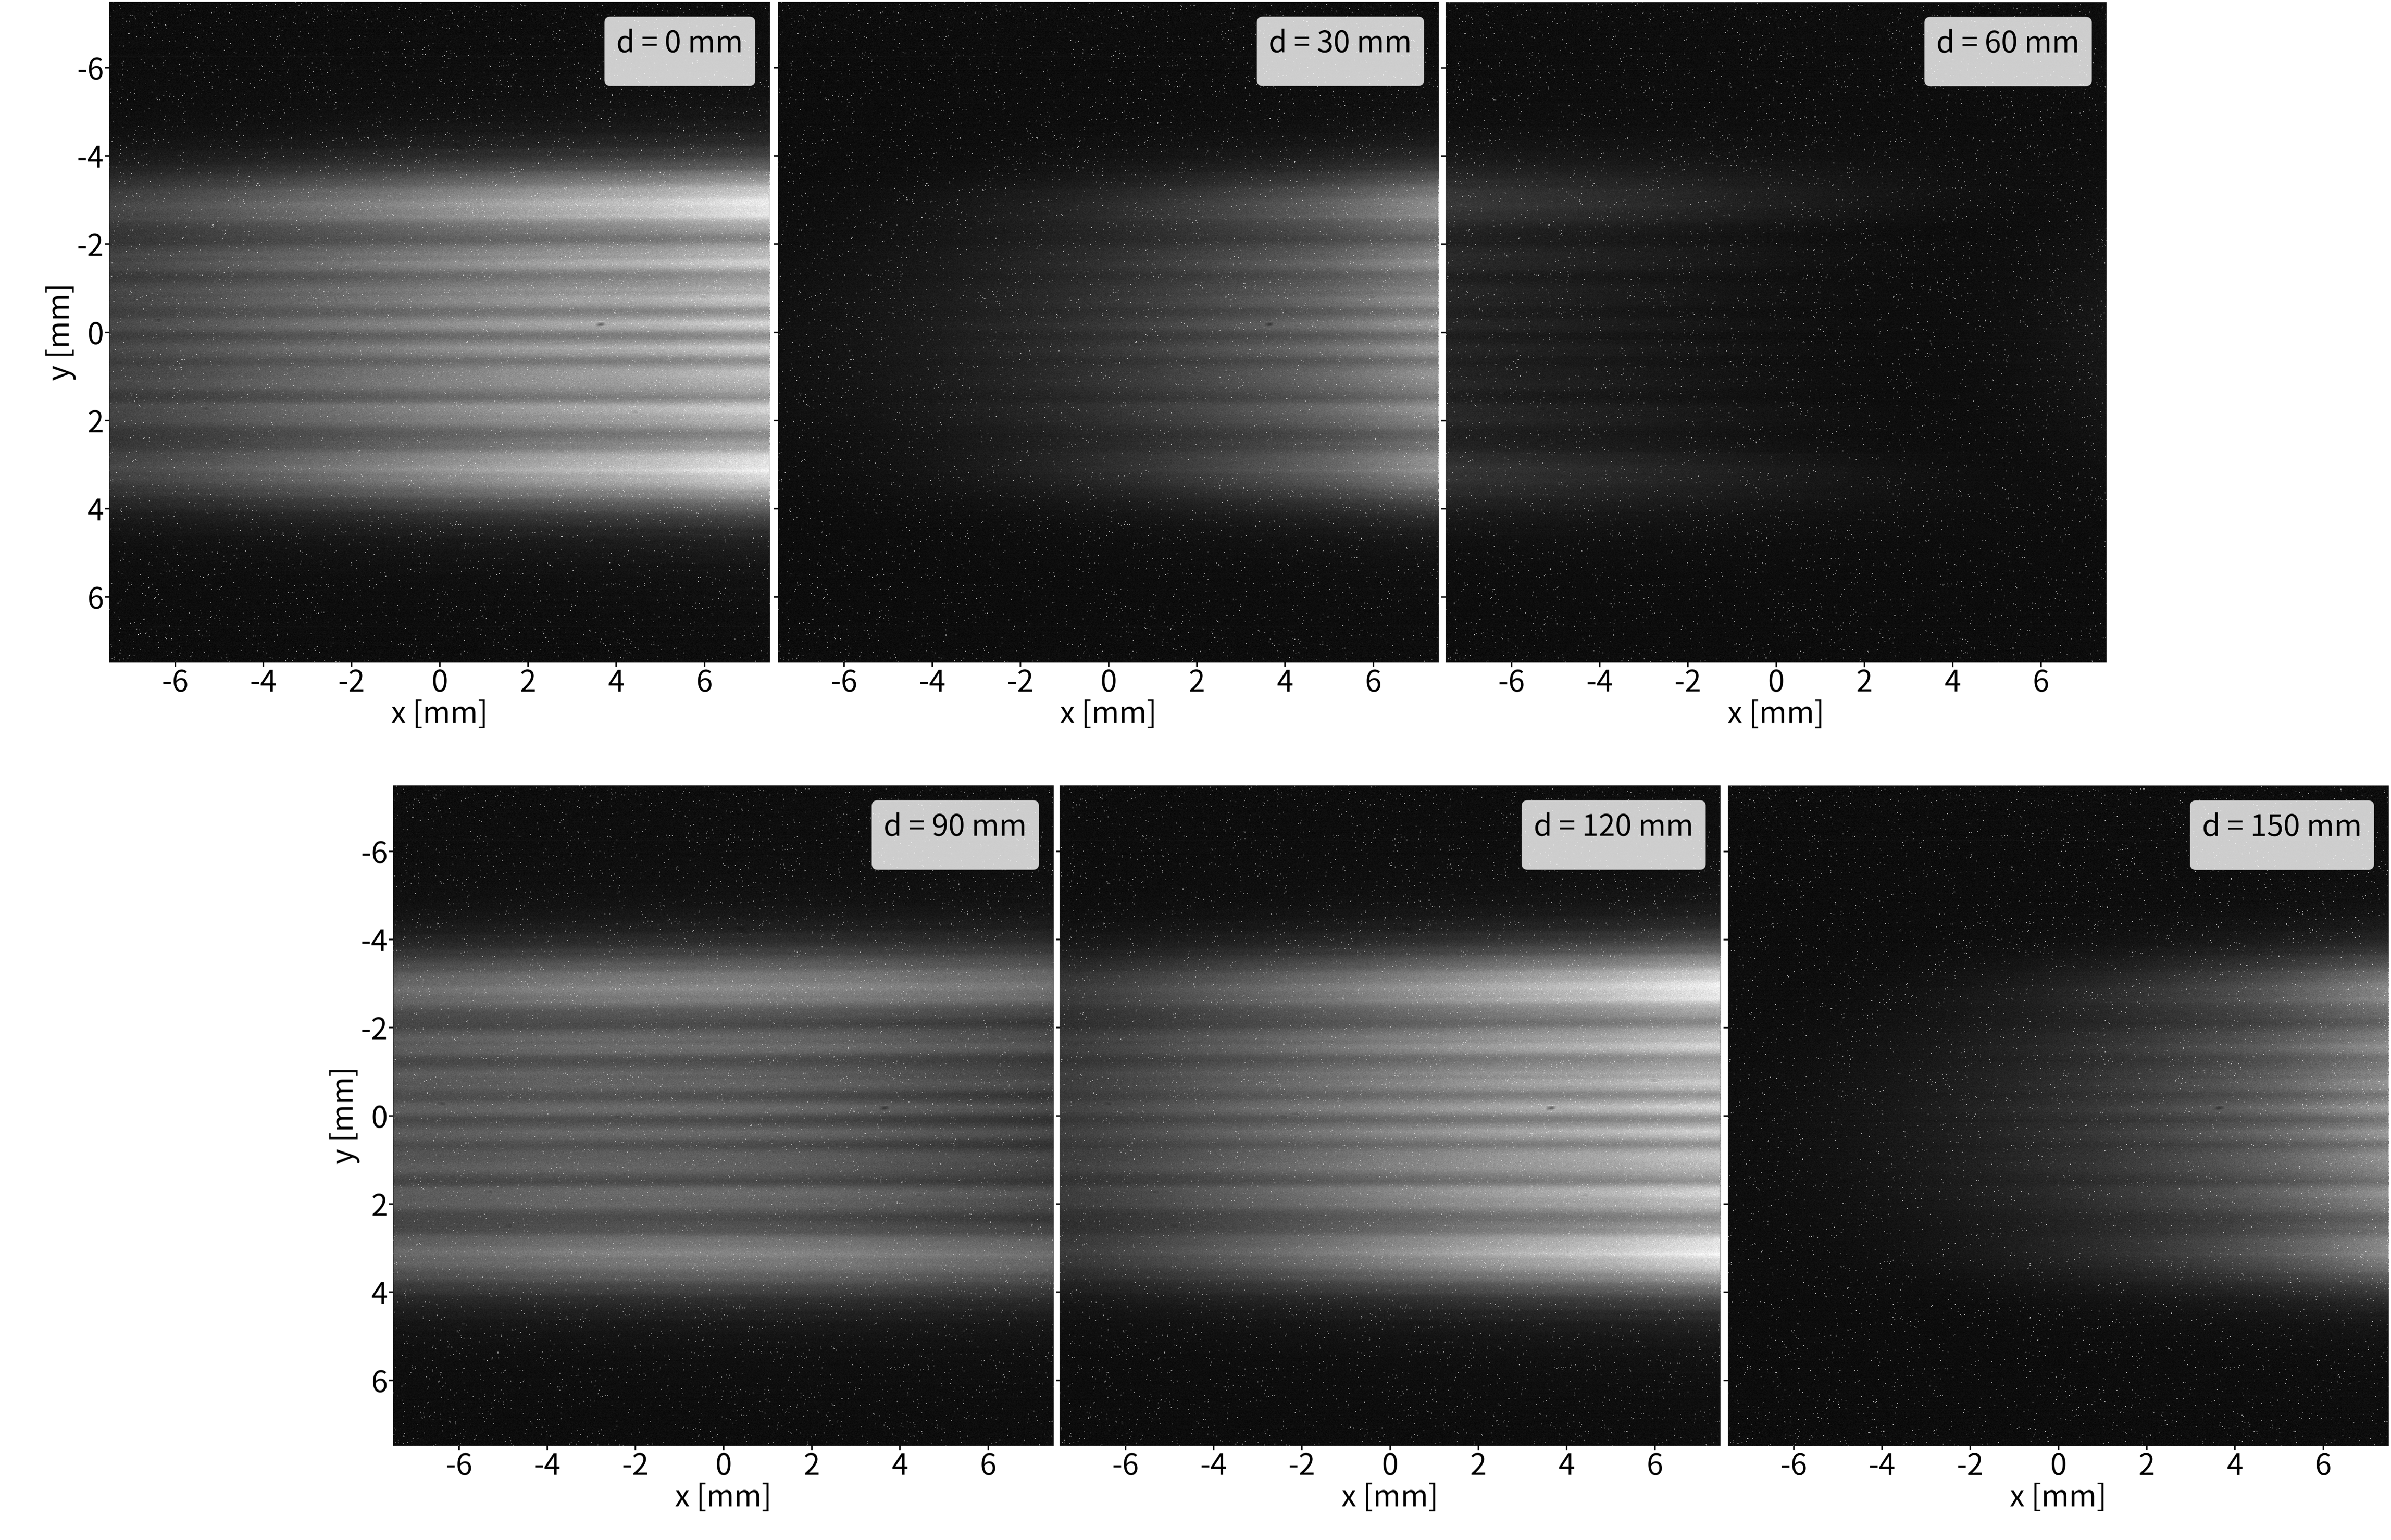
\includegraphics[width=0.8\linewidth]{image/4-images.png}
  \caption[干渉による画像の変化]{2台のアンジュレータで得られた画像の変化}\label{images}
\end{figure}

較正波長404.65 nm、y軸方向の中心のピクセルの周期的変動を、アンジュレータの位置$d$に対してプロットした結果の例を示す。周期的変動がみられることがわかる。
\begin{figure}
  \centering
  \includegraphics[width=0.8\linewidth]{image/4-oscillation.png}
  \caption[アンジュレータ位置に対する振幅の変化]{アンジュレータ位置に対する振幅の変化。較正波長 404.65 nm、$y$ =0 mmのピクセルを選び、ピクセル値を$d$に対してプロットすると周期的変動が見られる。}
\end{figure}
%fittingの結果

\section{統計誤差の見積もり}
\noindent \textbf{\underline{解析}}\par
統計誤差の見積もりはブートストラップ法によって行う。
ブートストラップ法はデータから復元抽出を行い、その復元抽出データから統計量を計算することで統計量の分布を推定する手法である。
下流アンジュレータの位置に関してランダムに復元抽出を複数回行い、抽出されたデータの集合に対してフィッティングを行う。得られたパラメータの分布から統計誤差を見積もる。

また各パラメータ同士の相関もブートストラップ法の復元抽出データから求めることができる。
理想的には全てのパラメータ同士が相関を持たない。

\noindent \textbf{\underline{結果}}\par
ブートストラップ法による統計誤差の見積もりの結果を示す。100個の異なる復元抽出データから得られる
$\gamma$の分布を示す。この分布から求めた$\gamma$の平均値と標準偏差は
\begin{eqnarray}
  \gamma = 381.232 \pm 0.052
\end{eqnarray}
である。
\section{系統誤差の見積もり}
波長依存性と位置依存性による誤差が主要な系統誤差の要因と考えられる。
\subsubsection{波長依存性}
\noindent \textbf{\underline{解析}}\par
前節で求めた較正波長(404.65 nm)におけるエネルギー測定の結果に加えて、同じモデル関数を用いて異なる波長でのデータからエネルギーを求める。
各波長に対してブートストラップ法を用いて統計誤差を見積もる。
異なる波長に対するエネルギーの分布から、モデル関数や装置のもつ波長依存性による系統誤差を見積もる。

\noindent \textbf{\underline{結果}}\par
横軸を波長に、縦軸をその波長における$\gamma$の推定値としたグラフを図\ref{wldep}に示す。
\begin{figure}[h]
  \centering
  \includegraphics[width=0.8\linewidth]{image/4-wldep.png}
  \caption{エネルギーの推定値の位置依存性}\label{wldep}
\end{figure}

また、アクセプタンス全体における$\gamma$の分布の平均値および標準偏差は、
\begin{eqnarray}
  \gamma = 381.242 \pm 0.059
\end{eqnarray}

\subsubsection{位置依存性}
\noindent \textbf{\underline{解析}}\par
アンジュレータの位置によるエネルギーの推定値の違いを見積もる。
具体的には、アンジュレータの位置を4つの区間に分割し、各区間でエネルギーを求める。アンジュレータ位置に対する放射光関数の補正がどの程度の影響を持つかを見積もる。

\noindent \textbf{\underline{結果}}\par
横軸を4分割の区間のインデックス、縦軸を各区間で得られた$\gamma$の推定値としたグラフを図\ref{posdep}に示す。
\begin{figure}[h]
  \centering
  \includegraphics[width=0.8\linewidth]{image/4-posdep.png}
  \caption[アンジュレータ位置に対するエネルギーの推定値]{アンジュレータ位置に対するエネルギーの推定値。split index 1がもっとも上流であり、アンジュレータの可動範囲の最上流を0 mm としたときに
  split index 1は 0 mm から205 mm、split index 2は205 mmから410 mm、split index 3は415 mmから620 mm、split index 4は620 mmから825 mmの範囲を示す。}\label{posdep}
\end{figure}

\subsubsection{エネルギー依存性}
180、195、210 MeVの3つのエネルギーの結果を表に示す。

\end{document}